\documentclass[aps,prl,reprint,superscriptaddress]{revtex4-1}

%--- PACKAGES ---%
% \usepackage[T1]{fontenc}
\usepackage{graphicx}
\usepackage[usenames,dvipsnames]{color}
\usepackage{amsmath,amssymb}
\usepackage{bm}
\usepackage{upgreek}
\usepackage{xspace}
\usepackage{units}
\usepackage{hhline}
\usepackage[vskip=0pt]{quoting}
\usepackage[colorlinks,urlcolor=blue,citecolor=blue,linkcolor=blue]{hyperref}
\graphicspath{{figures/}}
\renewcommand{\arraystretch}{1.5}

%--- TEXT SHORTCUTS ---%
\newcommand{\etal}{et~al.\xspace}
\newcommand{\Rb}{$^{87}$Rb\xspace}
\newcommand{\qmagic}{q_{\text{magic}}\xspace}
\newcommand{\qRmagic}{q_{R,\text{magic}}\xspace}
% \newcommand{\lundblad}{Phys. Rev. Lett. \textbf{118}, 2xxxxx (2017)}
\newcommand{\lundblad}{arXiv:1706.xxxx}

%--- TEXT OPERATORS ---%
\newcommand{\reffig}[1]{\mbox{Fig.~\ref{#1}}}
\newcommand{\refeq}[1]{\mbox{Eq.~(\ref{#1})}}
\newcommand{\refsec}[1]{\mbox{Sec.~(\ref{#1})}}
\newcommand{\note}[1]{\textcolor{ForestGreen}{[\textrm{#1}]}} % Make editorial notes red

%--- MATH OPERATORS ---%
\newcommand{\upd}{\text{d}}
\newcommand{\totalD}[2]{\frac{\upd #1}{\upd #2}}
\newcommand{\partialD}[2]{\frac{\partial #1}{\partial #2}}
\newcommand{\vecop}[1]{\hat{\mathbf{#1}}\xspace}
\newcommand{\expect}[1]{\langle #1 \rangle}
\newcommand{\abs}[1]{\vert #1 \vert \xspace}
\newcommand{\bra}[1]{\langle #1 \vert \xspace}
\newcommand{\ket}[1]{\vert #1 \rangle \xspace}
\newcommand{\braket}[2]{\langle #1 \vert #2 \rangle \xspace}
\newcommand{\vect}[1]{\mathbf{#1}\xspace}
\newcommand{\uvect}[1]{\hat{\mathbf{#1}}\xspace}
\newcommand{\epvec}{\hat{\mathbf{\epsilon}}\xspace}
\newcommand{\jvect}{\mathbf{\tilde{E}}\xspace}
\newcommand{\ham}{\mathcal{H}}

% Underscores in text (from http://tex.stackexchange.com/a/38720)
\catcode`_=12
\begingroup\lccode`~=`_\lowercase{\endgroup\let~\sb}

\begin{document}

\title{Continuously observing the spectrum of a dynamically decoupled spin-1 quantum gas}

\author{R.\,P.~Anderson}
\author{M.\,J.~Kewming }
\author{L.\,D.~Turner}
\affiliation{School of Physics \& Astronomy, Monash University, Victoria 3800, Australia.}

\date{\today}

\begin{abstract}
Quantum systems can be engineered so that their spectra are sensitive to a particular measurand whilst simultaneously impervious to parasitic fluctuations of an environment.
Here we use a minimally perturbative atom-light interface to study the dressed-state energy spectrum of a spin-1 quantum gas continuously and in-situ.
The spins are coupled by a radio-frequency field, whose amplitude sets the frequency band in which oscillating magnetic fields manifest a linear measurand, and we probe the energy spectrum while the system evolves unitarily.
By varying a symmetry-breaking parameter of the Hamiltonian, we find a regime in which two of the dressed states are maximally insensitive (up to fourth-order) in magnetic field fluctuations that are slow compared to the dressed-state splittings.
Moreover, we demonstrate the predictive power of our continuous probe to tune the measurement band and optimize the dynamical decoupling.
This robust system shares the useful hallmarks of quantum metrology platforms; the states are thus termed ``pseudo-clock'' states in a co-published result by Lundblad~\emph{et al.} (Phys. Rev. Lett. \textbf{118}, 2xxxxx (2017)) and are candidates for band-tunable magnetometry and color charge analogues in quantum gases. 
\end{abstract}

\maketitle

\section{Introduction}
\label{sec:introduction}
\begin{itemize}
    \item Minimally insensitive states in other systems, e.g. $\ket{F=1,m=-1} \leftrightarrow \ket{F=2,m=+1}$ at $B=3.23\unit{G}$, and variants thereof (including those insensitive to Rabi frequency variations reported on at Otago in 2016).
    \item Wide utility of these states for clocks, magnetometers (including microwave, e.g. Treutlein), quantum computing, etc.
    \item General message of making the eigenspectrum insensitive to one thing while retaining sensitivity to another; quantum version of common-mode rejection.
    \item Dynamical decoupling in this context.
    \item Motivate continuous measurement, especially in context of measurement bandwidth; it doesn't make sense to measure something in kHz--MHz band using a shot-based ($0.1\unit{Hz}$ or less) readout. Why? Can't react, can't feedback, can't always assume periodicity/repeatability.
    \item From magnetometry perspective, breaking rotational symmetry is bad because you want there to be no anisotropy to the sensitivity. How does this relate to this work?
    \item The parameter $q$ has been tuned using static magnetic fields and with microwave ac Stark shifts of an off-resonantly driven hyperfine transition, to e.g. to traverse the magnetic phase space of a spinor quantum gas, driving quantum quenches, etc.    
\end{itemize}

\begin{figure}
    \centering
    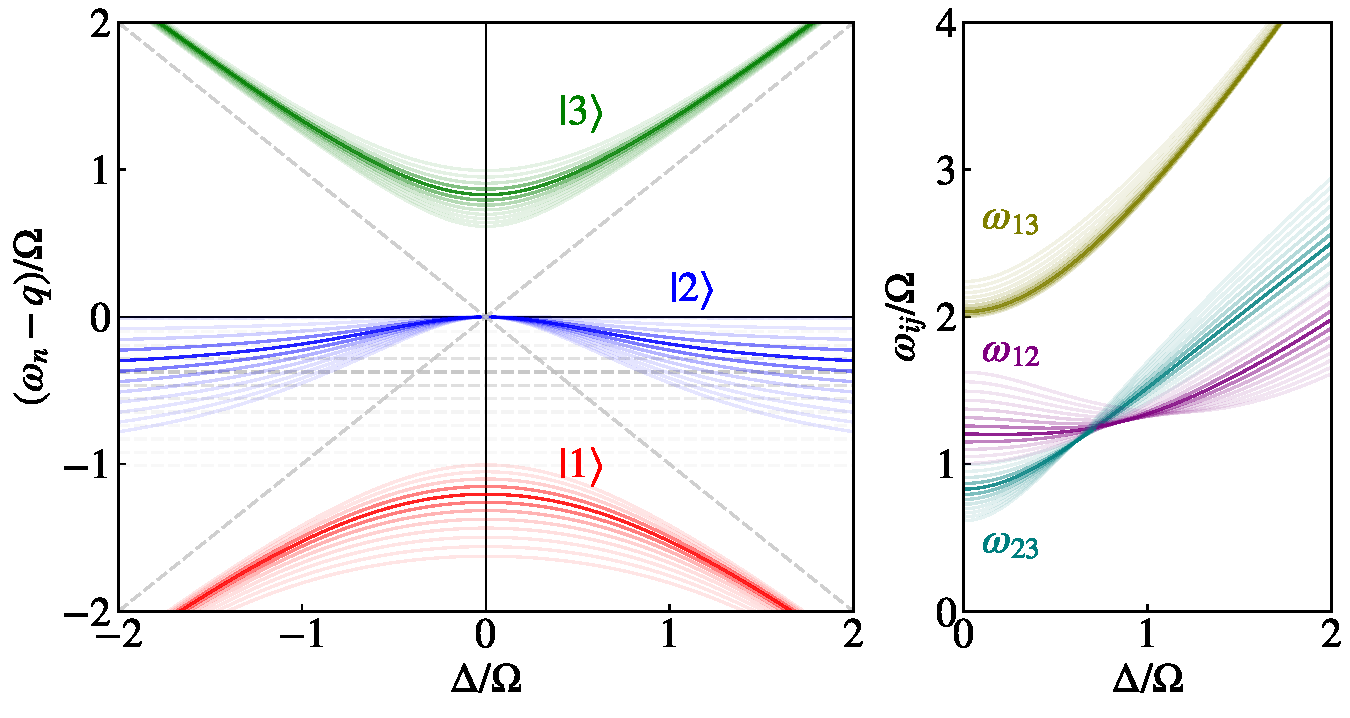
\includegraphics[width=\columnwidth]{figure_1.pdf}
    \caption{
    \label{fig:eigensystem_schematic}
        (Color online)
        Energy spectrum and splittings of a radiofrequency coupled spin-1 for various $q(B)\in[0,\Omega]$.
        The transparency of each curve is proportional to the distance of the quadratic shift $q$ from $\qmagic\approx 0.348\Omega$.
        (Left) Energies $\omega_n$ of dressed states $\ket{n}=\ket{1}$, (red) $\ket{2}$ (blue), and $\ket{3}$ (green) normalized to the rf-coupling strength (Rabi frequency) $\Omega$ as a function of detuning $\Delta(B)=\omega_{\text{rf}}-\omega_L(B)$,
        Dashed lines indicate the energies of uncoupled states ($\Omega=0$) in a frame rotating at $\omega_{\text{rf}}$.
        (Right) Splittings $\omega_{ij}$ of dressed states $\ket{i}$ and $\ket{j}$ as a function of detuning.
        When $q=\qmagic$ (bold curves), energies $\omega_1$ and $\omega_2$ share the same curvature, and their difference $\omega_{12}$ (right, purple) is minimally sensitive to detuning and thus magnetic field variations. 
    }
\end{figure}

\section{Background + random}
\label{sec:background}
\begin{itemize}
    \item Hamiltonians (quasi-static field along $z$, coupling field along $x$:
    \begin{align*}
        \hat{H}_{\text{lab}} &= \omega_L \hat{F}_z + q \hat{F}_z^2 + 2\Omega \cos (\omega_{\text{rf}} t) \hat{F}_x \\
        \Rightarrow \hat{H}_{\text{RWA}} &= -\Delta \hat{F}_z - q \hat{F}_z^2 + \Omega \hat{F}_x \, \text{, where} \\
        \omega_L(B) &\equiv (E_{m=-1} - E_{m=+1})/2\hbar \, \text{, and} \\
        q(B) &\equiv (E_{m=+1} + E_{m=-1} - 2 E_{m=0})/2\hbar
    \end{align*}
    are the Larmor frequency and quadratic shift, respectively, which can be gleaned from the Breit-Rabi equation. The rf Rabi frequency $\Omega = \gamma B_{\text{rf}}/2$ and detuning $\Delta(B) = \omega_{\text{rf}} - \omega_L(B)$.
    \item At low magnetic field strengths, $\omega_L \propto B$ and $q \propto B^2$, and for our parameters we are justified in taking $\omega_L = \gamma B$ and $q = q_Z B^2$, where $\gamma = 2\pi \times 702379\unit{Hz/G}$ is the gyromagnetic ratio for \Rb $F=1$ and $q_Z = 2\pi \times 71.89\unit{Hz/G^2}$.
    \item For most of the analysis presented here (with $\omega_L$ and $q$ defined as above) these proportionalities need not be met, or the results, e.g. value of $\qmagic$ require a small correction. 
    \item For $q=0$, $\hat{H} \propto \vect{B} \cdot \hat{\vect{F}}$ and is thus a generator of rotations, but $q \hat{F}_z^2 \neq 0$ breaks the $\text{SU}(2)$ symmetry of $\hat{H}$.
    \item We vary the magnetic field to affect a change in the detuning of $\Delta \in [0, 2\Omega]$, the domain of \reffig{fig:eigensystem_schematic}(B).
    \item Variations in $B \mapsto B_0 + \Delta B$ of order $B_{\text{rf}} = 2\Omega/\gamma$ affect the detuning linearly, \emph{viz.} $\Delta \mapsto \Delta - \gamma \Delta B$, and do not affect $q$ at all for sufficiently small field strengths.
    \item Indeed, our data corroborate this since we measure $q(B(t))$ across the calibration sweep and find it to be $\sigma(q)/(2\pi) = 20\unit{Hz}$ on average (alternatively, inferring $q$ from $\omega_L$ via Breit-Rabi gives $\sigma(q)/(2\pi) = 1.3\unit{Hz}$).
    \item Thus the horizontal axis in \reffig{fig:eigensystem_schematic} is a proxy for $\Delta B$, and $\omega_{12}$ at $q=\qmagic$ is has leading-order quartic sensitivity to $\Delta B$.
    \item At high fields ($B\approx 30\unit{G}$) this approximation is no longer valid; $q \approx \qmagic$ varies appreciably across $\Delta B \in [0, B_{\text{rf}}]$ and e.g. $\omega_{12}$ has weak linear dependence on $\Delta B$~\cite{lundblad_pseudo_2017}.
    \item \emph{On varying $\Omega$ or $q$ to change $q_R=q/\Omega$:}
    For a given static magnetic field, $q_R$ can be modified via the Rabi frequency. However, this is not what is represented in \reffig{fig:eigensystem_schematic}, as the normalization of the horizontal and vertical axes would vary for each $q_R$. Importantly, the insensitivity of $\omega_{12}$ to detuning only gets better for increasing $\Omega$ in absolute terms; if the rf amplitude is unlimited, use it. However, doing so also modifies the absolute dressed state splittings on resonance, and thus the bandwidth of the dressed spin-1 as an ac magnetometer. The take home message is then: use as high an rf amplitude as you can afford (or want to tune the ac-band to), and then modify $q_R$ via $q$ to realize the pseudo-clock states.
    \item \textit{Transitions between dressed states:} $\ket{1} \leftrightarrow \ket{2}$ and $\ket{2} \leftrightarrow \ket{3}$ driven by fields oscillating along $y$ or $z$ near frequencies $\omega_D \mp q_D$, respectively. Alternatively, $\ket{1} \leftrightarrow \ket{3}$ driven by fields oscillating along $x$ near frequency $2\omega_D$. This is very different to the fully polarized bare states $\ket{m=\pm 1}$, which are coupled by a single-photon transition as this would conserve neither photon number nor angular momentum. There is no such restriction on the dressed states however as they are neither eigenstates of $\hat{F}_z$ nor photon number. 
\end{itemize}
\textit{Lab frame eigenstates:}
\begin{itemize}
    \item mean splitting $\omega_L$; quadratic shift $q$.
    \item Pairwise coupling between $\ket{m=-1} \leftrightarrow \ket{m=0}$ and $\ket{m=0} \leftrightarrow \ket{m=+1}$ via $\hat{F}_x$ and/or $\hat{F}_y$, i.e. affected by fields transverse to the static field oscillating near $\omega_L$.
\end{itemize}
\textit{Dressed states on resonance:}
\begin{itemize}
    \item Dressed Larmor frequency:
    \begin{align*}
        \omega_D \equiv (\omega_3 - \omega_2)_{\Delta=0}/2 &= (\omega_{12} + \omega_{23})_{\Delta=0}/2 \\ &= \sqrt{\Omega^2 + q_D^2}\, .
    \end{align*}
    \item Dressed quadratic shift:
    \begin{align*}
        q_D &\equiv (\omega_3 + \omega_1 -2\omega_2)_{\Delta=0}/2 \\
            &= (\omega_{23}-\omega{12})_{\Delta=0}/2\\ 
            &= -q/2 \, .
     \end{align*}
    \item Thus $\Omega = \sqrt{\omega_{12} \omega_{23}}_{\Delta=0}$ and $q_D = (\omega_{23} - \omega_{12})_{\Delta=0}/2$, both of which can be attained from the dressed sideband splittings on resonance.
    Such high-bandwidth measurement of $\Omega$ (magnetic field oscillating along $x$ with amplitude $B_{\text{rf}}$ and frequency $\omega_L$) allows (in principle) closed-loop control of $\Omega$ using the atoms.
    \item For $q=0$ (low-field limit), the dressed states at $\Delta=0$ are eigenstates of $\hat{F}_x$, and: (i) the spectrum has vanishing linear sensitivity to magnetic fields, with the leading quadratic sensitivity (as in spin-$1/2$), and (ii) fields along $y$ or $z$ oscillating near the Rabi frequency $\Omega$ drive transitions between different $\ket{m_x}$ states. \note{Cite other dressed-ception papers on both of these.}
    \item Curvature of the dressed-state energies can be evaluated using perturbation theory;
    \[
    \partialD{^2\omega_n}{\Delta^2} = \sum_{k \neq n} \frac{\abs{\bra{k} \hat{F}_z \ket{n}}^2}{\omega_n - \omega_k} \, .
    \]
    \item Thus the curvature of the dressed-state splittings can be found. In particular, the dimensionless curvature of $\omega_{12}$ is (presuming $\abs{\partial q / \partial \Delta} \ll 1$) 
    \begin{align*}
    \partialD{^2(\omega_{12}/\Omega)}{(\Delta/\Omega)^2} &= \Omega \partialD{^2\omega_{12}}{\Delta^2} \\ &= -\frac{3 q_R \sqrt{4 + q_R^2} - q_R^2 - 2}{2 \sqrt{4 + q_R^2}} \, .
    \end{align*}
    This vanishes when $q = \qRmagic$, given by
    \[
    \qRmagic = \sqrt{(3\sqrt{2} - 4)/2} \approx 0.348 \, .
    \]
    \item Similarly, perturbation theory can be used to show that the third-order derivatives of $\omega_n$ with respect to detuning all vanish when $\abs{\partial q / \partial \Delta} \approx \abs{\gamma^{-1} \partial q / \partial B} \ll 1$, and thus the leading sensitivity to detuning (and thus $B$) is fourth-order. This validates the choice of our phenomenological even-polynomial model for fitting to $(\Delta B(t), \omega_{12}(t))$ data extracted from Faraday spectrograms.
    \item The above can be quantified by noting that $\gamma^{-1} \partial q / \partial B = 2 B q_Z / \gamma \lesssim 10^{-3}$ for $B \lesssim 5\unit{G}$.
    \item Near $q = \qmagic$, the ratio of the Rabi frequency to the Larmor frequency is approximately:
    \begin{align*}
        \frac{\Omega}{\omega_L} &= \frac{B_\text{rf}}{B_0} \\
                                &\approx \frac{q_z B_0}{\sqrt{2} \gamma \, \qRmagic} \\
                                &= 2.1\times10^{-4} B_0 \, ,
    \end{align*}
    with $B_0$ is in Gauss.
    Thus for $B_0 \lesssim 5\unit{G}$, $\Omega/\omega_L \lesssim 10^{-3}$ and the rotating-wave approximation is justified. 
\end{itemize}

\section{apparatus}
\label{sec:apparatus}
Our spinor quantum gas apparatus~\cite{wood_magnetic_2015} and Faraday atom-light interface are described in greater detail elsewhere~\cite{martijn_faraday_2017}.
We prepare an ultracold gas of approximately $10^6$ \Rb atoms in a crossed-beam optical dipole trap ($\lambda=1064\unit{nm}$).
The three Zeeman states $\ket{m=-1,0,+1}$ of the lowest hyperfine ($F=1$) ground state are coupled using a radiofrequency field with $\Omega/(2\pi) \leq 100\unit{kHz}$, generated by a single-turn coil placed immediately atop the glass vacuum cell, fed by an amplified radiofrequency source generated using direct-digital synthesis.
A component of the spin (e.g. $\expect{\hat{F}_x}$) transverse to the static magnetic field direction (along $z$) rotates the polarization of an off-resonant probe beam via the paramagnetic Faraday effect.
By tuning the probe to a magic-zero wavelength at $\lambda = 790.0\unit{nm}$, and ensuring it is linearly polarized, the probe exerts no scalar or vector light shift on the atoms.
The former would enact a dipole force on the cloud, perturbing its total density, whereas the latter would be manifest as a fictitious magnetic field and gradient, dephasing the collective spin~\cite{wood_measurement_2016}.
We detect the Faraday rotation of the probe light using a shot-noise limited balanced polarimeter, with bandwidth up to $8\unit{MHz}$, and record the signal using an AlazarTech \textsc{ATS9462} digitizer ($16$-bit, $180\unit{MS/s}$)
\footnote{The maximum Larmor frequency and thus static magnetic field we can detect Faraday rotation at is limited by the bandwidth of the detector.}.
Upon applying the radiofrequency (rf) dressing field, $\abs{\expect{\hat{F}_x}} > 0$ and the signature of the coupled spin-1 system is a Faraday signal frequency modulated (FM) about a carrier at the Larmor frequency.
The frequency difference of each FM sideband from the carrier is a calibration-free measure of each dressed state splitting $\omega_{ij}$.
As we seek to appraise the robustness of the rf-dressed states to varying magnetic fields, we apply a time dependent $\Delta B(t)$ and observe the dynamical change in the frequency composition of the Faraday signal using the short-time Fourier transform, or spectrogram.
The time-dependent magnetic field shift $\Delta B(t)$ is the sum of an applied linear ramp and the parasitic background fluctuations at the power-line frequency of $50\unit{Hz}$ and its odd harmonics, and typically ranges from $0$ ($\Delta = 0$, resonance) to $B_{\text{rf}}$ ($\Delta = 2\Omega$), \emph{cf.} \reffig{fig:eigensystem_schematic}.
For each realization (or `shot') of the experiment, we directly calibrate this time-dependent field using ac magnetometry; an rf $\pi/2$-pulse (rather than continuous coupling) initiates Larmor precession of the collective spin the $x$--$y$ plane, and the Faraday signal is composed of two tones, at $\omega_\pm = \omega_L \pm q$.
For $q \, \tau_f \geq 2\pi$, where $\tau_f$ is the length of the overlapping spectrogram windows, the two tones are spectrally resolved and their mean and difference yields the instantaneous $\omega_L(t)$ and $q(t)$, the former of which is used to find $\Delta B(t)$ by inverting the Breit-Rabi equation~\cite{ramsey_molecular_1963}. 
The experiment is synchronized to the AC power line; the harmonic composition of which varies little between contiguous shots ($20\unit{s}$ apart), and thus the measured $\Delta B(t)$ and $q(t)$ from the calibration shot serve as a good proxy for the values experienced by the atoms in the subsequent rf-dressed shot.

\bibliography{dressed_faraday}
   
\end{document}
